%%%%%%%%%%%%%%%%%%%%%%%%%%%%%%%%%%%%%%%
% Deedy - One Page Two Column Resume
% LaTeX Template
% Version 1.3 (22/9/2018)
%
% Original author:
% Debarghya Das (http://debarghyadas.com)
%
% Original repository:
% https://github.com/deedydas/Deedy-Resume
%
% v1.3 author:
% Zachary Taylor
%
% v1.3 repository:
% https://github.com/ZDTaylor/Deedy-Resume-Reversed
%
% IMPORTANT: THIS TEMPLATE NEEDS TO BE COMPILED WITH XeLaTeX
%
% This template uses several fonts not included with Windows/Linux by
% default. If you get compilation errors saying a font is missing, find the line
% on which the font is used and either change it to a font included with your
% operating system or comment the line out to use the default font.
%
%%%%%%%%%%%%%%%%%%%%%%%%%%%%%%%%%%%%%%
%
% TODO:
% 1. Add various styling and section options and allow for multiple pages smoothly.
%
%%%%%%%%%%%%%%%%%%%%%%%%%%%%%%%%%%%%%%
%
% CHANGELOG:
% v1.3:
% 1. Removed MacFonts version as I have no desire to maintain it nor access to macOS
% 2. Switched column ordering
% 3. Changed font styles/colors for easier human readability
% 4. Added, removed, and rearranged sections to reflect my own experience
% 5. Hid last updated
%
% v1.2:
% 1. Added publications in place of societies.
% 2. Collapsed a portion of education.
% 3. Fixed a bug with alignment of overflowing long last updated dates on the top right.
%
% v1.1:
% 1. Fixed several compilation bugs with \renewcommand
% 2. Got Open-source fonts (Windows/Linux support)
% 3. Added Last Updated
% 4. Move Title styling into .sty
% 5. Commented .sty file.
%
%%%%%%%%%%%%%%%%%%%%%%%%%%%%%%%%%%%%%%%
%
% Known Issues:
% 1. Overflows onto second page if any column's contents are more than the vertical limit
% 2. Hacky space on the first bullet point on the second column.
%
%%%%%%%%%%%%%%%%%%%%%%%%%%%%%%%%%%%%%%


\documentclass[]{deedy-resume-reversed}
\usepackage{fancyhdr}
\usepackage{graphicx}

\pagestyle{fancy}
\fancyhf{}

\begin{document}

%%%%%%%%%%%%%%%%%%%%%%%%%%%%%%%%%%%%%%
%
%     LAST UPDATED DATE
%
%%%%%%%%%%%%%%%%%%%%%%%%%%%%%%%%%%%%%%
% \lastupdated

%%%%%%%%%%%%%%%%%%%%%%%%%%%%%%%%%%%%%%
%
%     TITLE NAME
%
%%%%%%%%%%%%%%%%%%%%%%%%%%%%%%%%%%%%%%
\namesection{Yiwei Wang}{ %\urlstyle{same}\href{http://example.com}{example.com}| \href{http://example2.co}{example2.co}\\
\href{mailto:john.doe@example.com}{yiwei03.wang@tum.de} | \href{tel:11111111111}{+49 15231306657}
}

%%%%%%%%%%%%%%%%%%%%%%%%%%%%%%%%%%%%%%
%
%     COLUMN ONE
%
%%%%%%%%%%%%%%%%%%%%%%%%%%%%%%%%%%%%%%

\begin{minipage}[t]{0.60\textwidth}

\section{Research Interests}
Currently interested in robotics combined with computer vision, foundation models, or learning-based control, to enable robots to autonomously and reliably perform manufacturing tasks.
\sectionsep


\section{Working Experience}

\runsubsection{Tutor}
\descript{10/2025 - current}

\location{Chair of Robotics, Artificial Intelligence and Real-Time Systems, TUM}
\vspace{0.2em}
Tutor for the lecture \textit{Fundamentals of Artificial Intelligence}

\vspace{0.5em}
\runsubsection{Tutor}
\descript{10/2024 - 02/2025, 10/2025 - current}

\location{Chair of Human-Machine Communication, TUM}
\vspace{0.2em}
Tutor for the lecture \textit{Signals and Systems}

\vspace{0.5em}
\runsubsection{Intern}
\descript{08/2024 - 12/2024}

\location{Munich Institute of Robotics and Machine Intelligence (MIRMI)}
\vspace{0.2em}
Assisted in building a tele-operation system for a robotic arm and training a diffusion policy, enabling the robotic arm to perform basic tasks.

\vspace{0.5em}
\runsubsection{Tutor}
\descript{09/2023 – 10/2023}

\location{Chair of Optimal Control, TUM}
\vspace{0.2em}
Tutor for the \textit{Preparatory Course EI 2023}
\sectionsep




\section{Scholarships}

\textbf{10/2022 - 09/2025} "Foreign Schools Programs" Scholarship\\
\quad \textbf{DAAD} (German Academic Exchange Service)

\vspace{0.2em}
\textbf{09/2019 - 06/2022} Full Scholarship (Top 2\% of the students)\\
\quad \textbf{CEFLS} (Chengdu Experimental Foreign Language School)
\sectionsep

\section{Projects}
\runsubsection{Bachelor Thesis in MIRMI}
\descript{05/2025 - 09/2025}
\location{Munich Institute of Robotics and Machine Intelligence (MIRMI)}

\vspace{0.2em}

• Built a framework that enables robots to learn long-horizon assembly from a human demonstration video and execute reactively, with Behavior Trees serving as the planning output and supervisory control structure in a dynamic environment.

\vspace{0.1em}
• Under Review, arxiv: https://arxiv.org/abs/2509.16611


\vspace{0.5em}
\runsubsection{Sensor Network Visualization}
\descript{10/2024 - 01/2025}
\location{Chair of Data Processing, TUM}
\vspace{0.2em}
• A teamwork that built a sensor network visualization system in Python for sensor data processing and visualization.\\
• Served as team leader and implemented the core logic and server-side components.

\vspace{0.5em}
\runsubsection{Soft Skill Program „Adveisor“}
\descript{12/2022 - 06.2023}
\location{Chair of Automatic Control Engineering, TUM}
\vspace{0.2em}
• A teamwork that built an automated cocktail-making machine combining hardware control with a touchscreen interface for real-time and customizable drink preparation. \\
• Contributed to software design and motor control using Arduino

\sectionsep

\end{minipage}
\hfill
\begin{minipage}[t]{0.32\textwidth}
\vspace{0em}  % 双栏基准线

\vspace{1em}
\begin{center}
  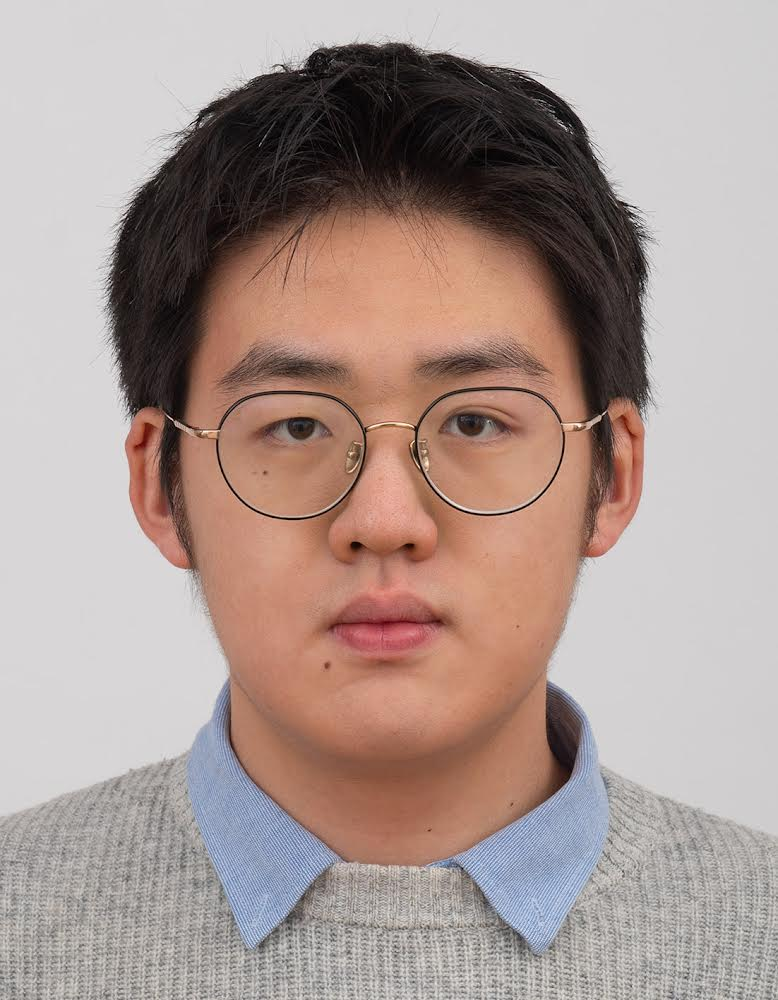
\includegraphics[width=0.6\linewidth]{Foto.png}
\end{center}


\section{Personal Information}
\textbf{Nationality}
Chinese

\textbf{Birth Date}
28.11.2003

\textbf{Birth Place}
Chongqing, China

\vspace{0.7em}
\section{Skills}
\subsection{Programming Languages}
C/C++, Python, Matlab
\sectionsep

\subsection{Languages}
English(C1), German(C1), Chinese
\sectionsep

\subsection{Softwares}
Arduino, CAD, and MATLAB Simulink
\sectionsep


\subsection{Technologies}
Git/Github, Linux, ROS, and Pytorch
\sectionsep

\vspace{0.7em}
\section{Education}

\subsection{Technical University of Munich}
\descript{10/2022 - 03/2026}
\descript{B.Sc. Electrical Engineering and Information Technology}
• Average grade 1.2/5, rank 3 within the best 2\%
% \location{Note: 1.2 / 5.0}
% \location{voraussichtlicher Abschluss: 03/2026}
\sectionsep

\subsection{Chengdu Experimental}
\subsection{Foreign Language School}

\descript{High School Diploma}
\descript{09/2019 - 06/2022}
• Top 2 \% of the students




\end{minipage}
\end{document}  \documentclass[]{article}